\documentclass{templateNote}
\usepackage{tcolorbox}
\usepackage{hyperref}
\usepackage{amsmath}
\usepackage{amssymb}
\usepackage{pdflscape}
\usepackage{soul}
\usepackage{media9}
\usepackage{adjustbox}

\begin{document}

\imagenlogoU{img/LogoElNube.png}
\linklogoU{https://github.com/MarceloPazPezo}
\linkQRDoc{https://github.com/MarceloPazPezo/MyRepo/tree/main/Icinf/Semestre\%207/Sistemas\%20de\%20Información/Test\%201}
\titulo{Test 1}
\asignatura{Sistemas de Información}
\autor{
    \indent
    Marcelo \textsc{Paz}
    \\
    \indent
    Nicolas \textsc{Gómez}
}
\portada
\margenes % Crear márgenes

\section{Sistemas de Información}
\begin{itemize}
    \item \textbf{Sistema:} Conjunto de partes que interactúan entre sí, para lograr un objetivo en común.
\end{itemize}
\begin{figure}[H]
    \centering
    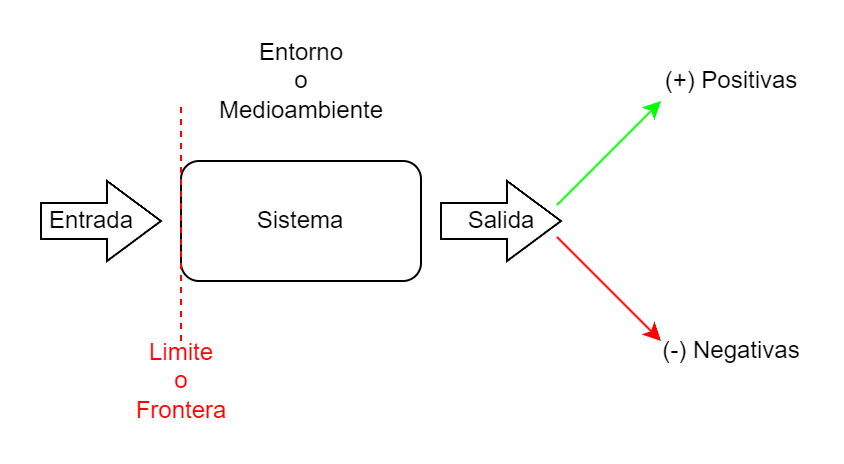
\includegraphics[width=0.9\textwidth]{diagramas/diagrama Sistema.png}
\end{figure}
Definiciones:
\begin{itemize}
    \item \textbf{Entrada:} Todo aquello que el sistema recoge de su entorno para cumplir con su objetivo.
    \item \textbf{Salida:} Todo aquello que el sistema entrega al entorno producto del cumplimiento de su objetivo.
    
    + Sistema se beneficia
    
    - Sistema no se beneficia
    
    Salida + > Salida -
\end{itemize}

\begin{itemize}
    \item \textbf{Sistema Abierto:} Es capaz de interactuar con el entorno por si solo.
    \item \textbf{Sistema Cerrado:} No es capaz de interactuar con el entorno por si solo.
    \item \textbf{Sinergia:} El todo es mas que las sumas de las partes. Las sumas de las partes cumplen un objetivo.
    \item \textbf{Conglomerado:} Conjunto de partes que no interactuán entre si.
    \item \textbf{Entropía:} Grado de desorden.
    \item \textbf{Dato:} Hecho conocido que no tiene valor.
    \item \textbf{Información:} Un dato al que se le agrega significado y utilidad.
    \item \textbf{Conocimiento Tácito:} Conocimiento que no se ve, como lo que esta en la mente de las personas.
    \item \textbf{Conocimiento Explícito:} Conocimiento que se puede ver, como textos o apuntes.
    \begin{itemize}
        \item Fácil de transmitir.
        \item Fácil de transpasar.
        \item Para transformar conocimiento tácito en explícito utilizando la documentación del conocimiento.
    \end{itemize}
    \item \textbf{Estrategia:} Es un camino a seguir para poder llegar al objetivo deseado.
    \item \textbf{Misión:} Razón de ser de la empresa.
    \item \textbf{Visión:} Sueño/Idea de llegar a ser.
    \item \textbf{Tecnologias de información:} Permiten desarrollar sistemas.
    \item \textbf{Recursos y capacidades:} El sistema no logra nada sin los recursos y capacidades.
    \item \textbf{Procesos:} Cosas que se hacen para convertir una entrada en salida.
    \item \textbf{Estructura:} Como se organiza.
    \item \textbf{Cultura:} Forma de hacer las cosas.
\end{itemize}

\begin{landscape}
\begin{figure}[H]
    \centering
    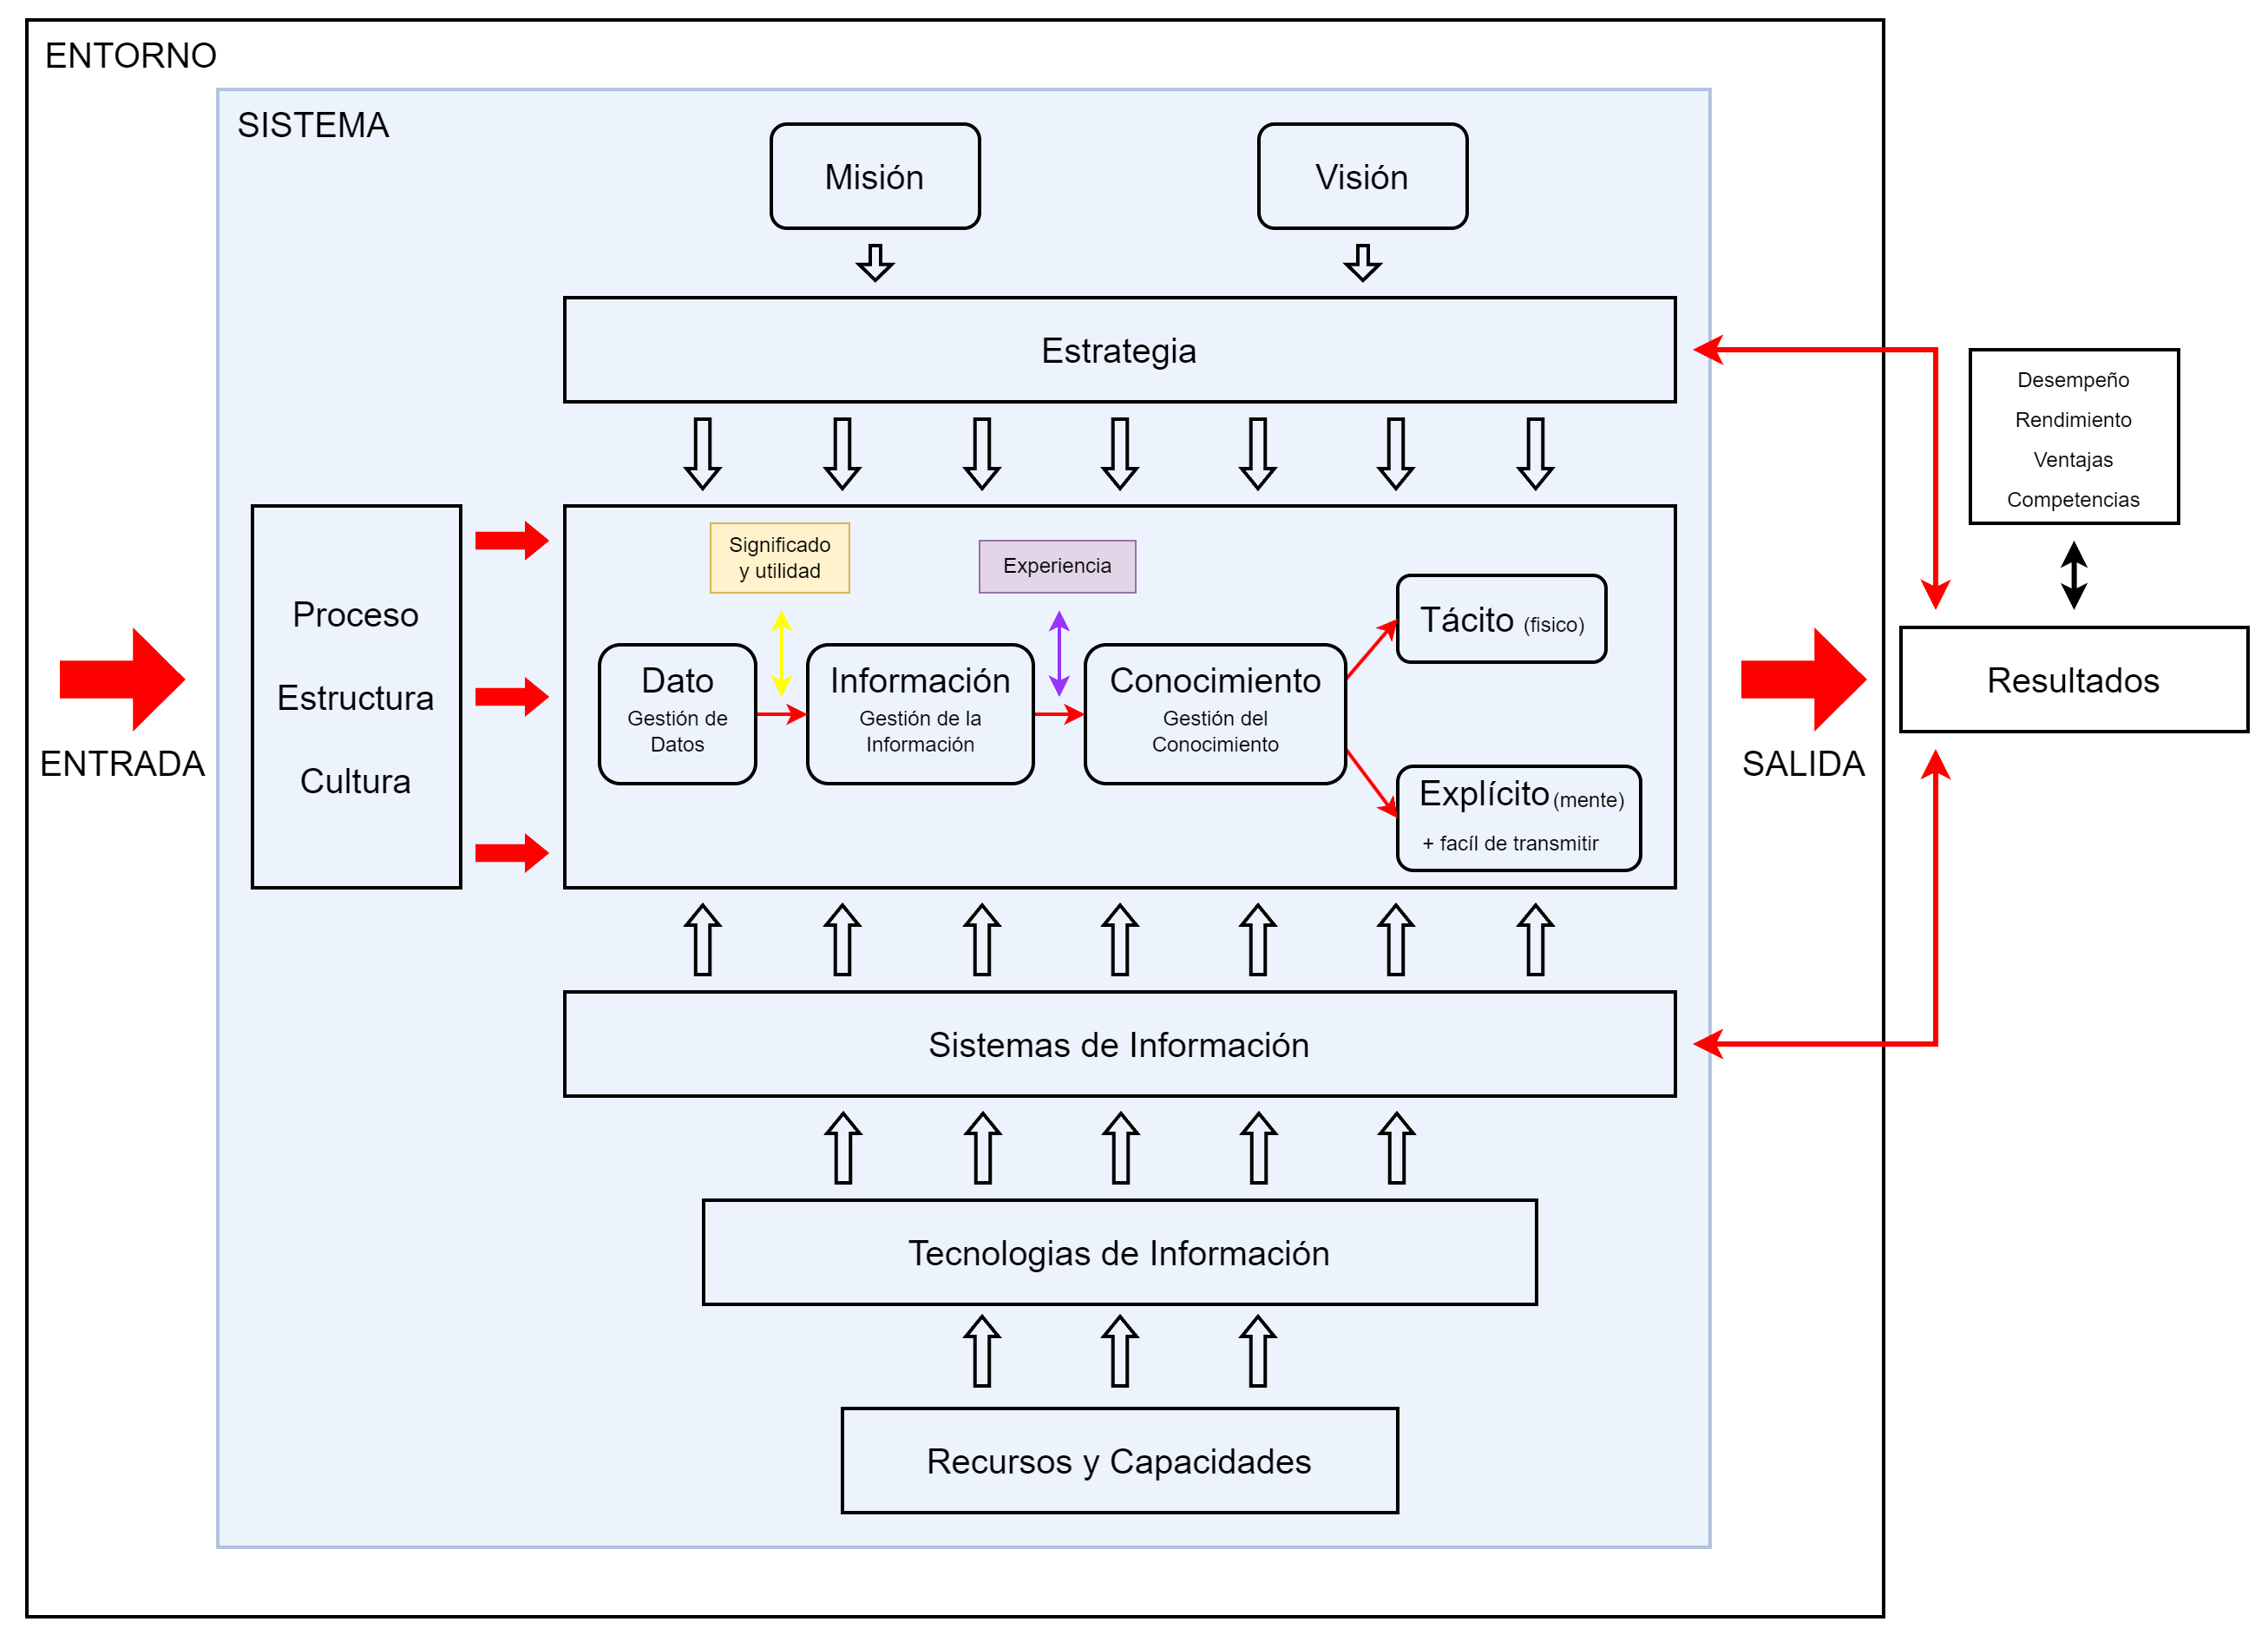
\includegraphics[width=1.35\textwidth]{diagramas/digramaCompleto.png}
\end{figure}
\end{landscape}

\newpage
\section{Piramide de Anthony}
\indent
Siempre encontramos 3 niveles:
\begin{figure}[H]
    \centering
    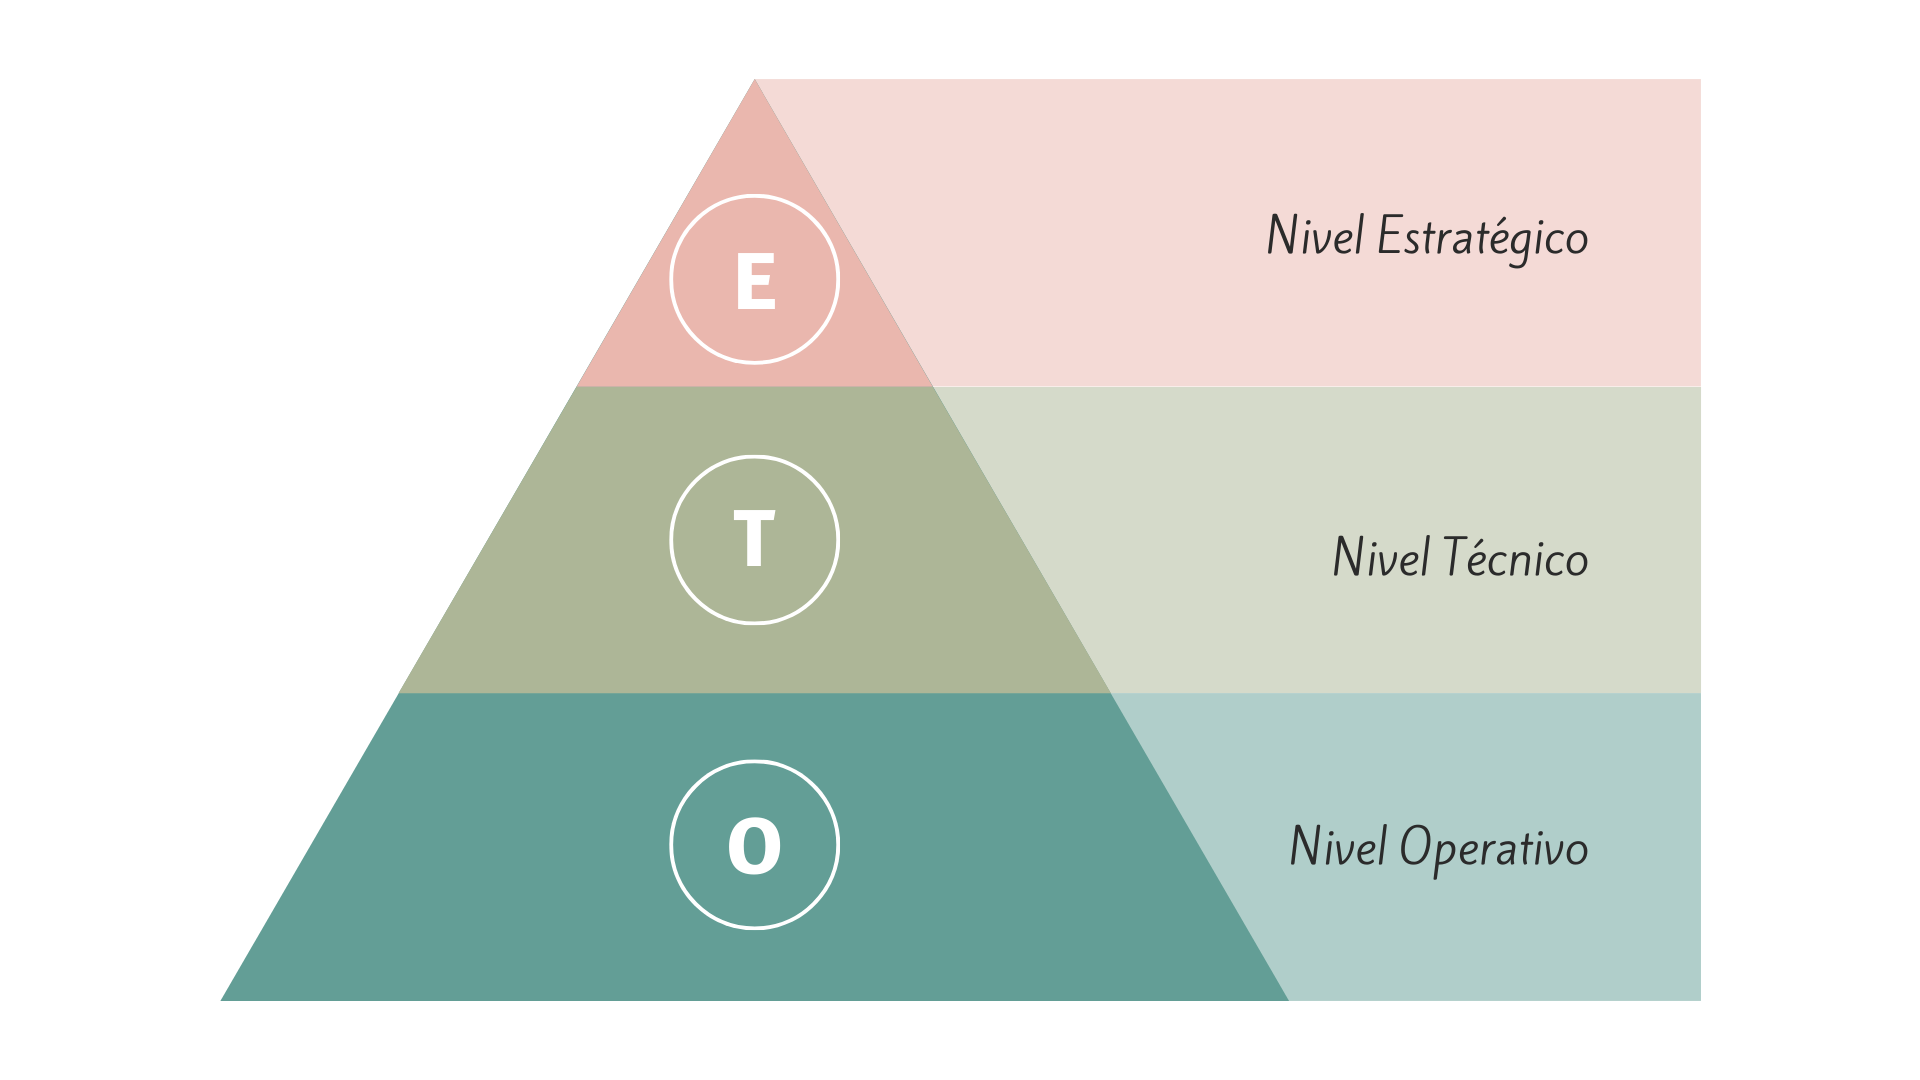
\includegraphics[width=0.7\textwidth]{img/PiramideAnthony.png}
    
    \textbf{Agradecimientos a Nicolas Gómez}
\end{figure}
\begin{itemize}
    \item \textbf{Nivel Estrategico:} Definición de Misión; Largo Plazo.
    \item \textbf{Nivel Táctico:} Control de gestión; Mediano Plazo.
    \item \textbf{Nivel Operativo:} Actividades rutinarias; No cambian; Corto Plazo.
\end{itemize}
\
\section{Características de la Información}
\begin{figure}[H]
    \begin{center}
        \noindent\adjustbox{center}{
            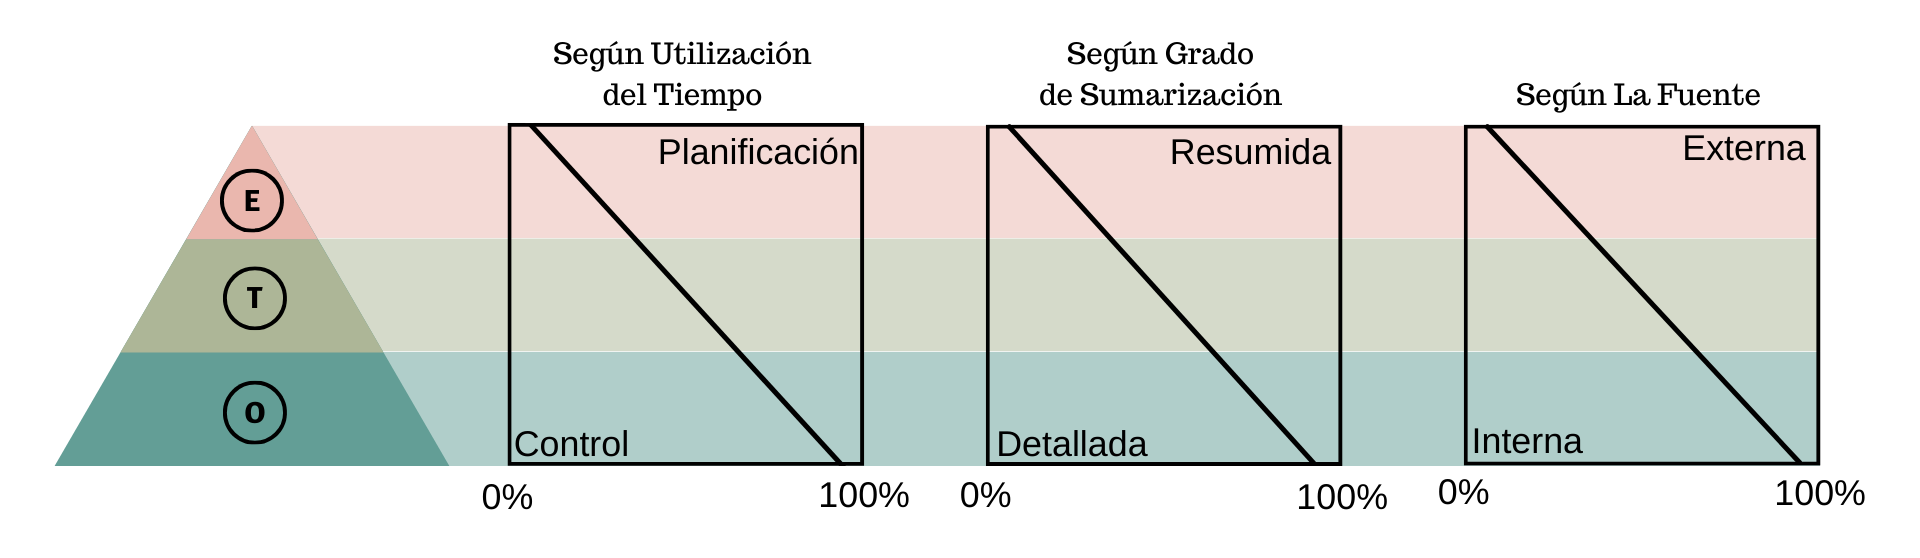
\includegraphics[width=1.2\textwidth]{img/PiramideAnthony2.png}
        }
        \textbf{Agradecimientos a Nicolas Gómez}
    \end{center}
\end{figure}
% \begin{itemize}
%     \item Según la utilización del tiempo.
%     \begin{itemize}
%         \item 
%         \item $\downarrow$ Información se utiliza para mayor control.
%     \end{itemize}
% \end{itemize}
 
\newpage
\begin{itemize}
    \item \textbf{Sistema de Información:} \hl{Conjunto formal de procesos} que operando sobre una \hl{colección de datos estructurados} recopila, elabora y distribuye (parte de) la información \hl{necesaria para la operación de dicha empresa} y para las actividades de \hl{dirección y control} correspondientes apoyando al menos en parte la toma de \hl{decisiones necesarias} para desempeñar las \hl{funciones y procesos} de acuerdo con la \hl{estrategia.}
    \begin{itemize}
        \item Un proceso es formal cuando esta bien definido, este proceso se puede estudiar.
        \item Un proceso es informal cuando no esta bien definido.
        \item Los datos estan estructurados según la necesidad de la empresa.
        \item Recopilación, elaboración y distribución $\rightarrow$ Sistema con entrada, proceso y salida.
    \end{itemize}
\end{itemize}

\section{Curva de Nolan}
\begin{figure}[H]
    \centering
    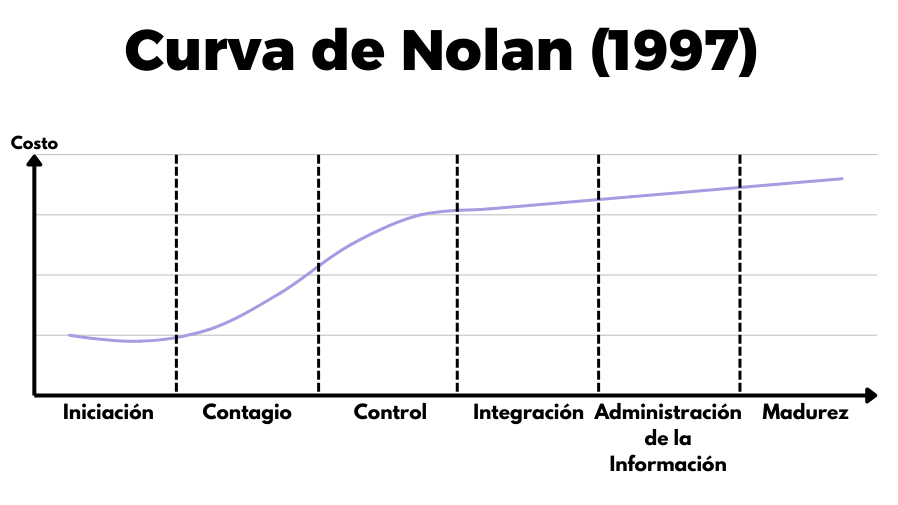
\includegraphics[width=0.7\textwidth]{img/CurvaDeNolan.png}
\end{figure}
*$Implementación \rightarrow Organización \rightarrow Dirección \rightarrow Control$
\\ \\
\textbf{Actualización de Curva de Nolan}
\begin{figure}[H]
    \centering
    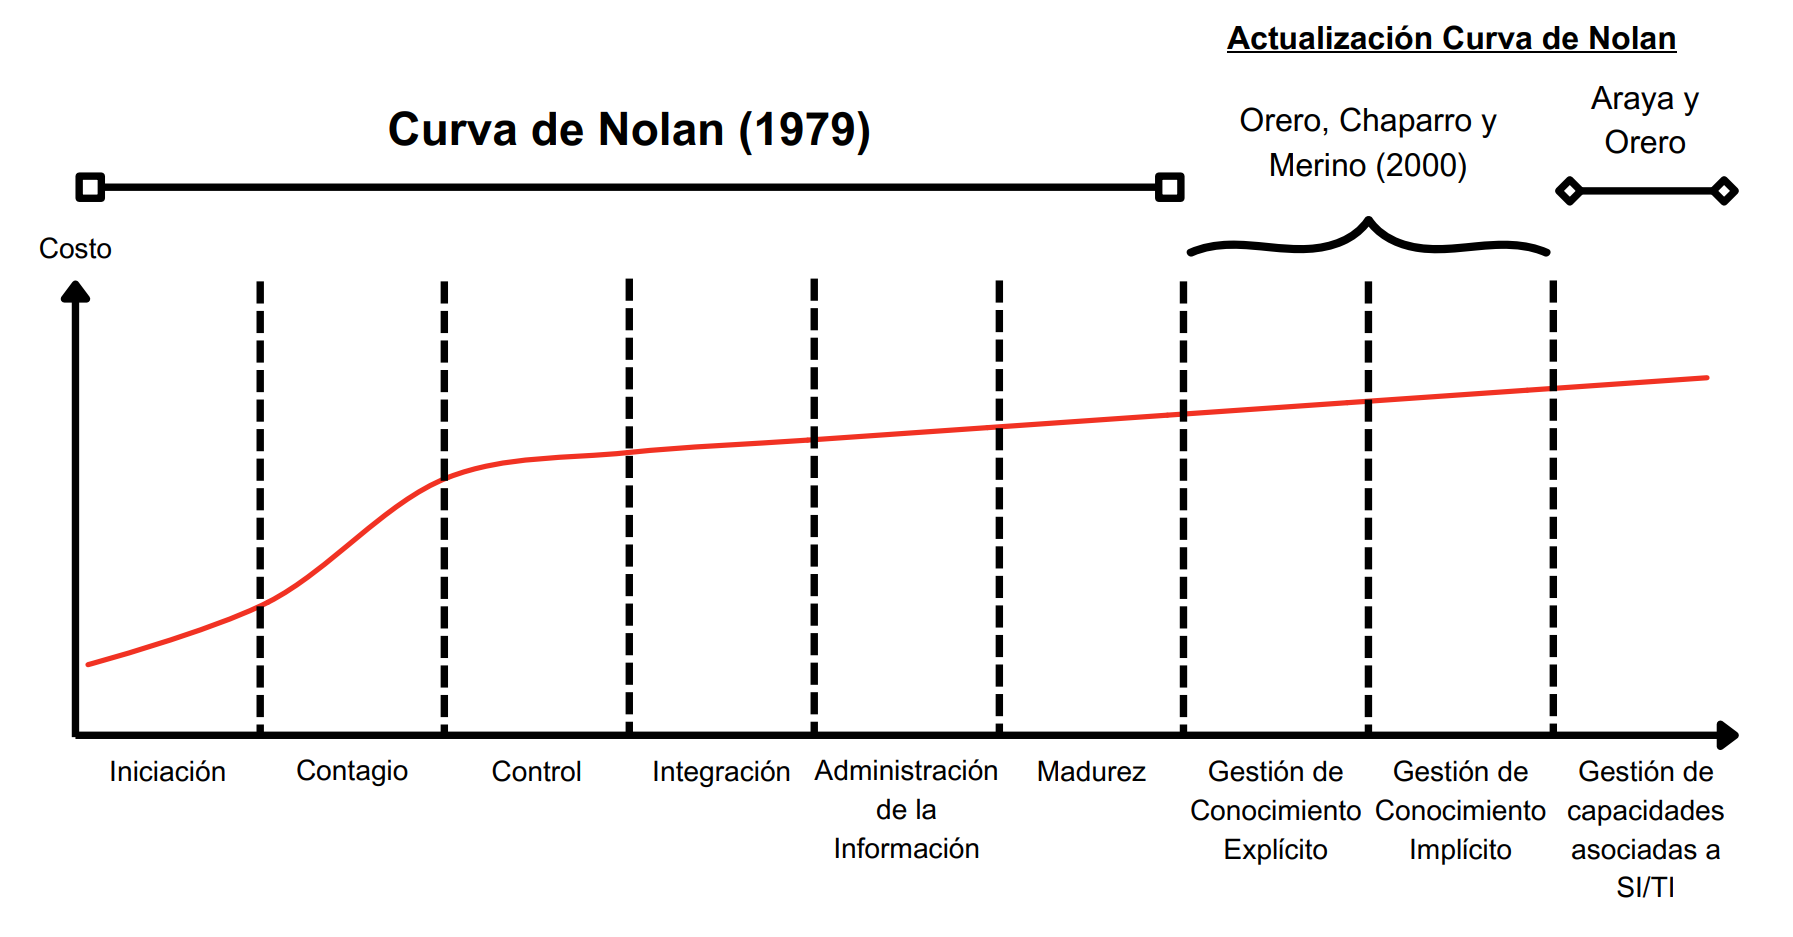
\includegraphics[width=0.9\textwidth]{img/CurvaDeNolanActualizada.png}
\end{figure}
\end{document}